To test the model, a cable with a pressure sensor has been put on the boat in order to capture the behaviour of the cable.



\section*{Boat specification}

The boat is a retrofitted version of the model Mini-12 and can be consider of the 2.4mR-class by the International Sailing Federation meaning is length is around 4 meters. It weigh around 300 kg.

To proceed to the measurement of the cable depth, a pressure sensor has been added and also an Arduino  Uno as  Analog to digital converter and send the sensor data to the computing unit a Raspberry Pi 3 Model B.

\begin{figure}[H]
\centering
    \begin{minipage}[b]{0.4\textwidth}
    \centering
    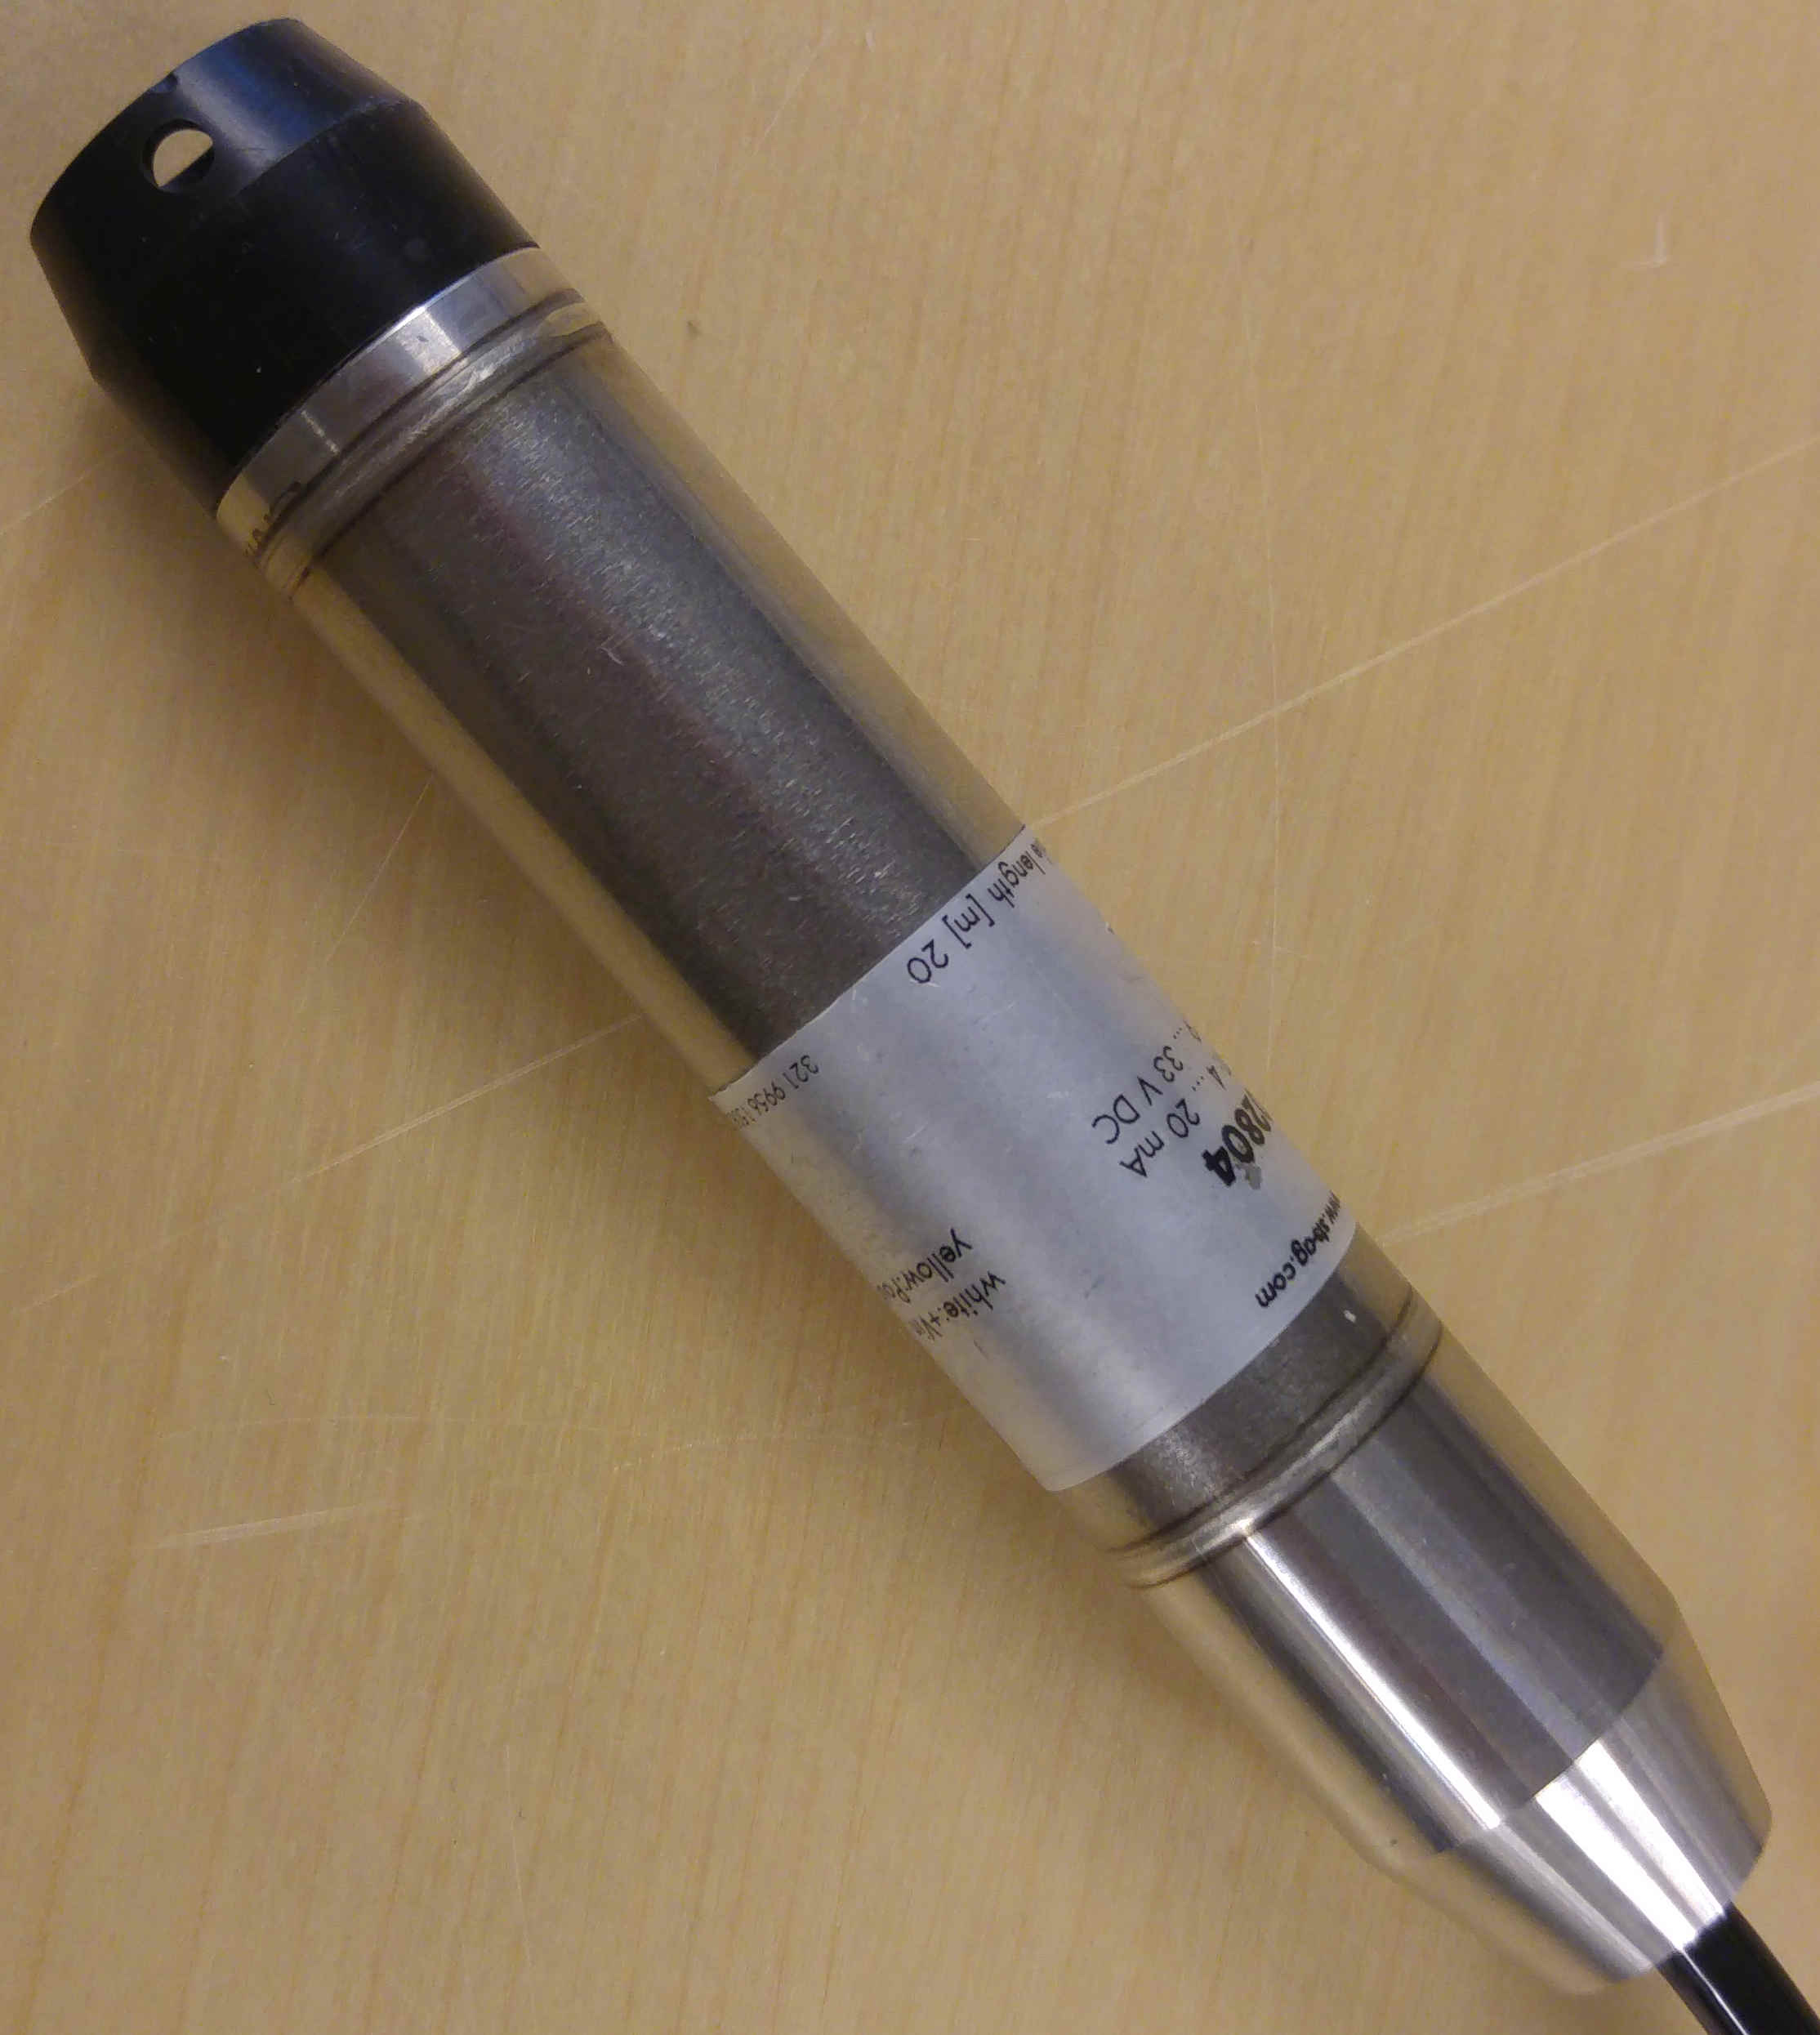
\includegraphics[scale=0.024,angle=0]{pressure_sensor.jpg}
    \caption{Pressure Sensor used to measure the depth of the cable.}
    \label{fig:pressure sensor}
    \end{minipage}
    \hfill
    \begin{minipage}[b]{0.45\textwidth}
    \centering
    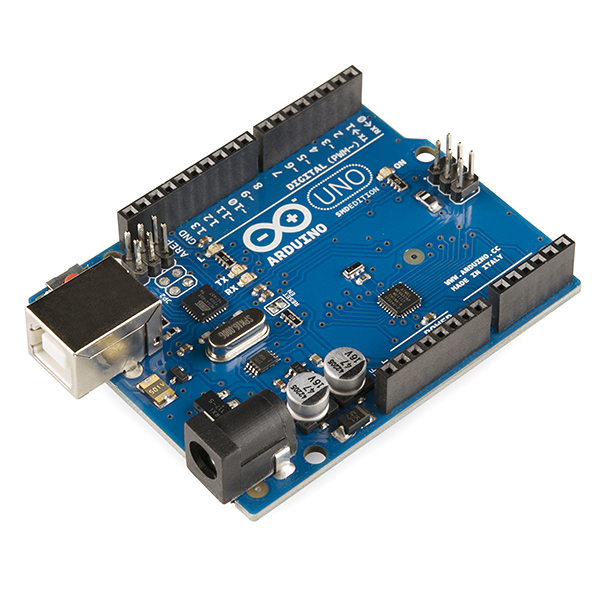
\includegraphics[scale=0.4,angle=0]{arduino_uno.jpg}
    \caption{Arduino Uno as a converter for the pressure sensor.}
    \label{fig:comp_depth_speed_2007}
    \end{minipage}
\end{figure}

The data was first received be an Xbee, a radio transmitter, and logged on a remote computer via Labview, but the data transfer was not reliable enough to get good interpretation of the results. Then the pressure sensor have been incorporated in the database (remote and local) , data is sent live to a web server to be saved and displayed via a 4G modem. 
Actuator

Battery

Raspberry V3

Arduino Uno 

pressure sensor

xbee 

labview  taken from before

maestro polulu
 radio receiver
 sensor current
\section{Test process}
The boat is a retrofitted one person sailing boat . 
First the gathered data will be compared with the old model for tuning. Then the test with cable will be compared to the new model.
Cant expect perfect result because the model of sailboat is not perfect, it only allow to design controller for the boat itself. The goal is the same here determine possibility for controller create a new model for cable (from profile determine from the cable is it doesn't effect to much the boat)
Tests has been realised to test the boat:

\begin{itemize}
\item Cable added on the hull of the boat (between 6 and 20 m)
\item Tapping a pressure sensor on the cable
\item Boat has to reach multiple waypoints while measuring the depth of the pressure sensor
\item Boat redo the same path without cable
\end{itemize}

To measure the depth of the cable a pressure sensor is put alongside it, the pressure sensor cable is smaller than 
the long one (3 meters in the water) so to compare to the simulation what is compare is the depth of the 3 meter mark on the boat or the depth of the end of the cable compared to the pressure sensor extrapolated to the length of the bigger cable.

\section{Validation of cable simulation}

First the depth of the pressure sensor will be compared to the depth of the simulation of the cable when taking the speed and position data.

\begin{figure}[H]
\centering
    \begin{minipage}[b]{0.4\textwidth}
    \centering
    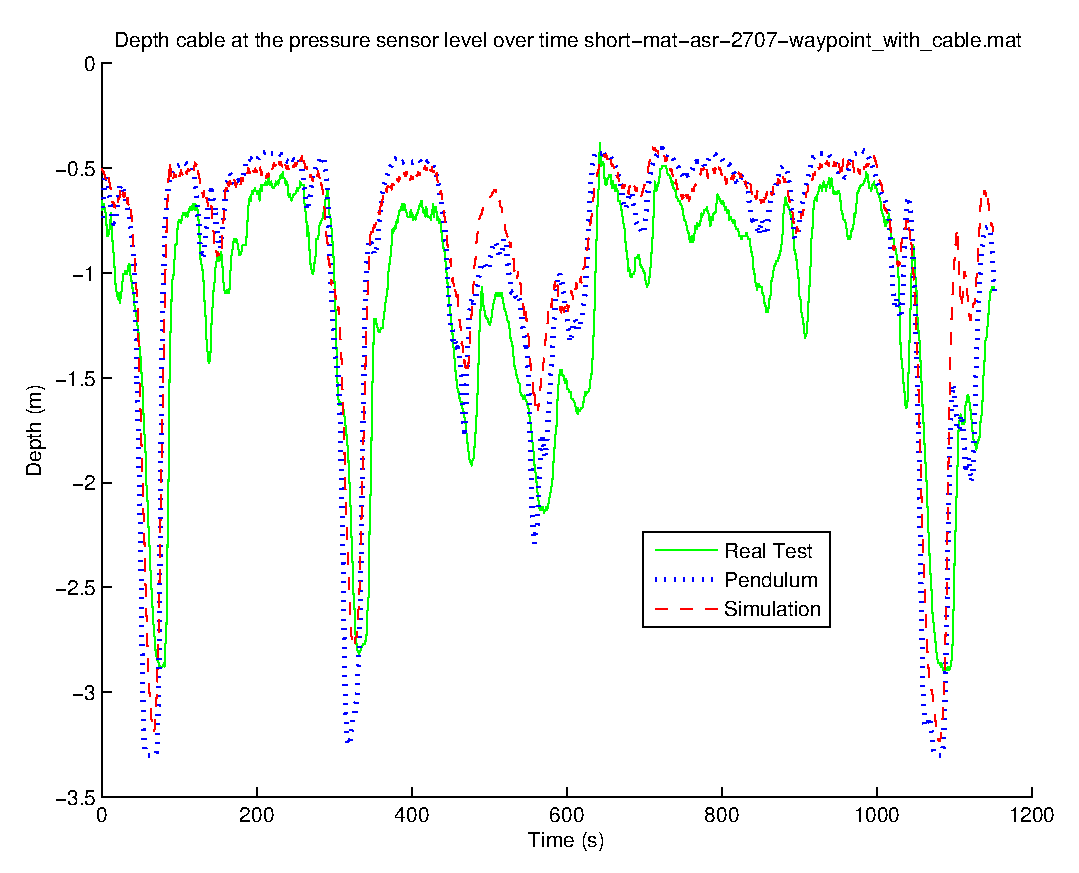
\includegraphics[scale=0.4,angle=0]{depth_time_2707}
    \caption{Comparison between depth of cable at the pressure sensor level in simulation and real test.}
    \label{fig:comp_depth_time_2007}
    \end{minipage}
    \hfill
    \begin{minipage}[b]{0.45\textwidth}
    \centering
    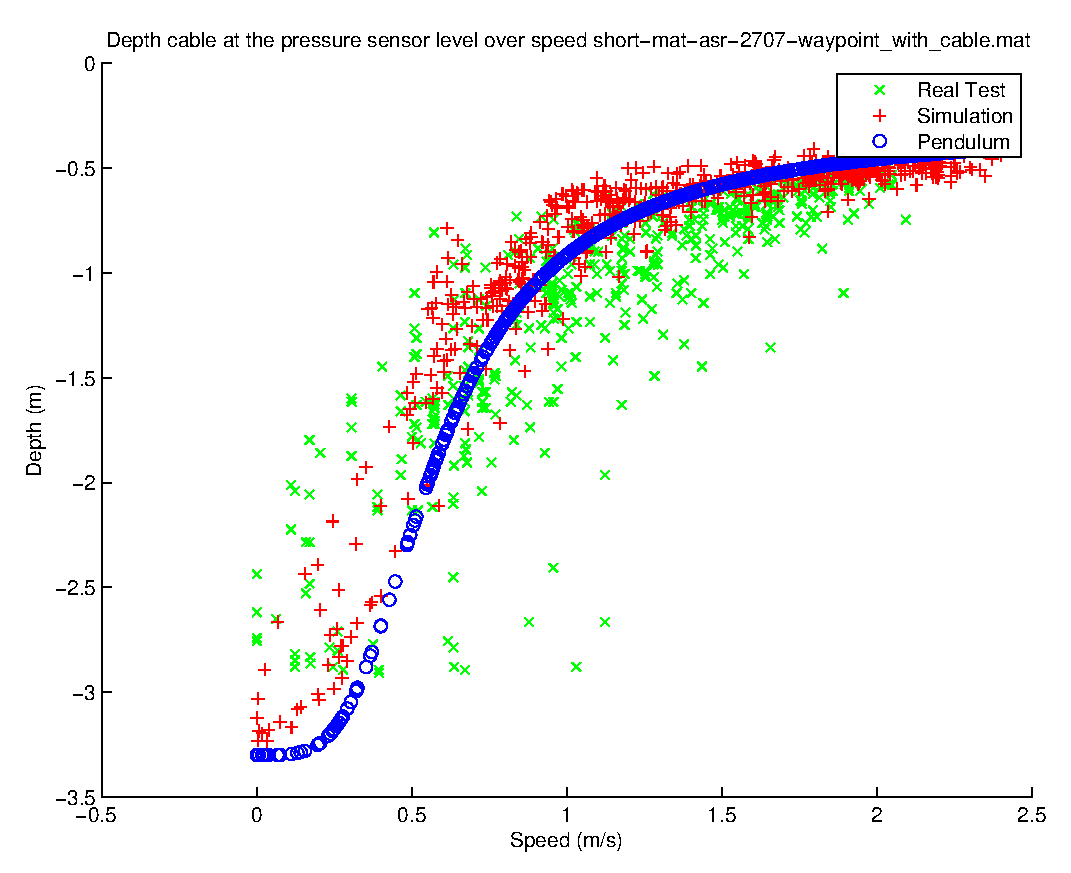
\includegraphics[scale=0.4,angle=0]{depth_speed_2707}
    \caption{Comparison of depth of cable at the pressure sensor level in function of speed between simulation and real test.}
    \label{fig:comp_depth_speed_2007}
    \end{minipage}
\end{figure}
